\documentclass[a4paper,12pt]{report}
%general packages
\usepackage[T2A]{fontenc}
\usepackage[utf8]{inputenc}
\usepackage[english,russian]{babel}
\usepackage{circuitikz}
\usepackage{wrapfig}
\usepackage{makecell}
\usepackage{tabularx}
\usepackage{graphicx}
\usepackage{gensymb}
\usepackage{cancel} %cancel symbol
\usepackage{amsmath,amsfonts,amssymb,amsthm,mathtools}
\usepackage[dvipsnames]{xcolor}


%\usepackage{epstopdf} %converting to PDF
%\usepackage{auto-pst-pdf}

%fancy header + geometry
\usepackage{fancyhdr}
\usepackage[a4paper,includehead,nomarginpar,left=15mm,right=15mm,top=15mm,headheight=10mm,bottom=20mm]{geometry}

%pgfplots
\usepackage{pgfplots}
\usepackage{pgfkeys}
\pgfplotsset{compat=1.12}
\usepackage{mathrsfs}

%multi column text
\usepackage{blindtext}
\usepackage{multicol}

%tikz (draw)
\usepackage{tikz}
\usepackage{pstricks-add}
\usetikzlibrary{intersections}
\usetikzlibrary{arrows.meta}
\usetikzlibrary{calc,angles,positioning}
\usetikzlibrary{arrows}
\usepackage{float}
\usepackage{filecontents}

%parskip settings
\parindent=0ex
\setlength{\parskip}{\baselineskip}%
\setlength{\parindent}{0pt}%

%fancy notation for sets
\newcommand{\R}{{\mathbb R}}
\newcommand{\N}{{\mathbb N}}
\newcommand{\fancy}[1]{{\mathbb{#1}}}
%sgn function
\DeclareMathOperator{\sgn}{sgn}

% intersection and union symbols
\newcommand{\uni}{\cup}
\newcommand{\inter}{\cap}
\newcommand{\re}{\text{Re}}
\newcommand{\const}{\text{const}}

\renewcommand{\footrulewidth}{0.4pt}

%\newcommand{\celsius}{$\ ^\circ C$}

%environments

\newtheorem{problem}{Задача}[]
\newenvironment{sol}{\paragraph{Решение}}{}
\renewcommand\thesection{\arabic{section}}

\usepackage{titlesec}
\titlespacing*{\section}
{0cm}{\baselineskip}{0pt}
\titlespacing*{\subsection}
{0pt}{0.1\baselineskip}{0.1\baselineskip}
\titlespacing*{\paragraph}
{0pt}{0.1\baselineskip}{\baselineskip}

\setcounter{secnumdepth}{0}

\begin{document}
	

\begin{titlepage}
	\begin{center}
		МОСКОВСКИЙ ФИЗИКО-ТЕХНИЧЕСКИЙ ИНСТИТУТ (НАЦИОНАЛЬНЫЙ ИССЛЕДОВАТЕЛЬСКИЙ УНИВЕРСИТЕТ) \\
		
		
		\hfill \break
		Факультет обшей и прикладной физики\\
		\vspace{2.5cm}
		\large{\textbf{Отчёт по лабораторной работе 1.2.5 <<Исследование прецессии уравновешенного гороскопа>>}}\\
		\hfill \break
		\\
	\end{center}
	
	\begin{flushright}
		Выполнил:\\
		Студент гр. Б02-304\\
		Головинов. Г.А.
	\end{flushright}
	
	\vspace{7cm}
	
	\begin{center}
		
\includegraphics[width=0.15\linewidth]{uni}
	\end{center}
	

	

	\vfill
	
	\begin{center} Долгопрудный, 2023 \end{center}
	
	\thispagestyle{empty}
	
\end{titlepage}


	\newpage
	%\pagenumbering{arabic}
    \pagestyle{fancy}

    \fancyhead{}
    \fancyfoot{}
    \fancyhead[L]{\rightmark}
    \fancyhead[R]{\thepage}
    \fancyfoot[R]{Работа 2.4.1. --- определение теплоты испарения жидкости}

    \section*{Аннотация}
        \paragraph*{Цель работы:} 1) измерение объёмов форвакуумной и высоковакуумной частей установки; 2) определение скорости откачки системы в стационарном режиме, а также по ухудшению и улучшению вакуума.
        \paragraph*{В работе используются:} вакуумная установка с манометрами: масляным, термопарным и ионизационным.
    \vspace{0.5cm}
    \hrule

    \section{Основные теоретические сведения}

    \subsection{Принцип работы ионизационного манометра}

    \begin{multicols}{2}
        Ионизационный манометр представляет собой трёхэлектродную лампу. Электроны испускаются накалённым катодом и увлекаются электрическим полем к аноду. Проскакивая за витки анода, электроны замедляются полем коллектора и возвращаются к катоду, а от него вновь увлекаются к аноду.

        Перед тем, как осесть на аноде они успевают много раз пройти расстояние между катодом и анодом, на этом пути они ионизируют молекулы газа. Ионы, образовавшиеся между анодом и коллектором, притягиваются его полем. По ионному току в цепи можно понять плотность молекул газа (она пропорциональна току), отсюда уже можно найти давление газа. 

        \begin{figure}[H]
            \centering
            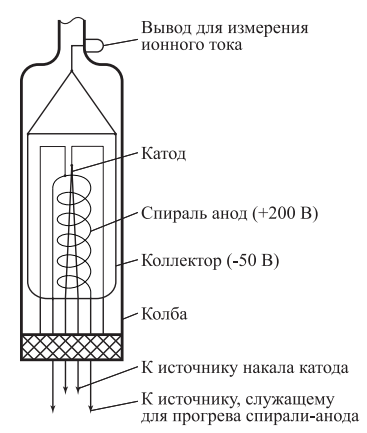
\includegraphics[width=0.7\columnwidth]{../img/ion_lamp.png}
            \caption{Схема ионизационной лампы.}
        \end{figure}
    \end{multicols}

    \hrule

    \newpage

    \subsection{Процесс откачки}

    \begin{multicols}{2}
        Пусть $W$ --- скорость откачки насосом, $Q_\text{д}$ --- количество газа, десорбирующегося с поверхности откачиваемого объема в единицу времени, $Q_\text{и}$ --- количество газа, проникающего в единицу времени извне, $Q_\text{н}$ --- поток газа, поступающего обратно из насоса. Все потоки $Q$ будем измерять в единицах $pV$.

        \begin{gather}
            -Vdp=(pW-Q_\text{д}-Q_\text{н}-Q_\text{и})dt \label{eq:1}
        \end{gather}

        При достижении предельного давления $p_\text{пр}$:
        \begin{gather*}
            \frac{dp}{dt}=0
        \end{gather*}
        значит
        \begin{gather}
            p_\text{пр}W=Q_\text{д}+Q_\text{н}+Q_\text{и}
        \end{gather}

        Обычно $Q_\text{и}$ --- постоянно, а два других потока слабо зависят от времени, поэтому скорость откачки $W$ можно считать постоянной. Чтобы отойти от предельного давления следует проинтегрировать \eqref{eq:1}:

        \begin{gather*}
            -V\int_{p_\text{пр}}^{p}\frac{dp}{p}=\int_{0}^{t}\left(W-\frac{\sum Q_i}{p}\right)dt \\
            p-p_\text{пр}=(p_0-p_\text{пр})\exp{\left(-\frac{W}{V}t\right)}
        \end{gather*}
        учитывая, что $p_\text{пр}\ll p_0$, получим:
        \begin{gather}
            p=p_0\exp{\left(-\frac{W}{V}t\right)}
        \end{gather}
        Постоянная откачки $\tau=V/W$ является мерой эффективности откачки системы.

    \end{multicols}

    \hrule

    \section{Обработка результатов измерений}

    \begin{multicols}{2}
        
    \end{multicols}
\end{document}
